%% March 2018
%%%%%%%%%%%%%%%%%%%%%%%%%%%%%%%%%%%%%%%%%%%%%%%%%%%%%%%%%%%%%%%%%%%%%%%%%%%%
% AGUJournalTemplate.tex: this template file is for articles formatted with LaTeX
%
% This file includes commands and instructions
% given in the order necessary to produce a final output that will
% satisfy AGU requirements, including customized APA reference formatting.
%
% You may copy this file and give it your
% article name, and enter your text.
%
%
% Step 1: Set the \documentclass
%
% There are two options for article format:
%
% PLEASE USE THE DRAFT OPTION TO SUBMIT YOUR PAPERS.
% The draft option produces double spaced output.
%

%% To submit your paper:
\documentclass[draft,linenumbers]{agujournal2018}
\usepackage{apacite}
\usepackage{url} %this package should fix any errors with URLs in refs.
%%%%%%%
% As of 2018 we recommend use of the TrackChanges package to mark revisions.
% The trackchanges package adds five new LaTeX commands:
%
%  \note[editor]{The note}
%  \annote[editor]{Text to annotate}{The note}
%  \add[editor]{Text to add}
%  \remove[editor]{Text to remove}
%  \change[editor]{Text to remove}{Text to add}
%
% complete documentation is here: http://trackchanges.sourceforge.net/
%%%%%%%


%% Enter journal name below.
%% Choose from this list of Journals:
%
% JGR: Atmospheres
% JGR: Biogeosciences
% JGR: Earth Surface
% JGR: Oceans
% JGR: Planets
% JGR: Solid Earth
% JGR: Space Physics
% Global Biogeochemical Cycles
% Geophysical Research Letters
% Paleoceanography and Paleoclimatology
% Radio Science
% Reviews of Geophysics
% Tectonics
% Space Weather
% Water Resources Research
% Geochemistry, Geophysics, Geosystems
% Journal of Advances in Modeling Earth Systems (JAMES)
% Earth's Future
% Earth and Space Science
% Geohealth
%
% ie, \journalname{Water Resources Research}

\journalname{Geohealth}


% tightlist command for lists without linebreak
\providecommand{\tightlist}{%
  \setlength{\itemsep}{0pt}\setlength{\parskip}{0pt}}



\usepackage{soulutf8}
\usepackage{float}
\usepackage{booktabs}
\usepackage{longtable}
\usepackage{array}
\usepackage{multirow}
\usepackage{wrapfig}
\usepackage{colortbl}
\usepackage{pdflscape}
\usepackage{tabu}
\usepackage{threeparttable}
\usepackage{threeparttablex}
\usepackage[normalem]{ulem}
\usepackage{makecell}
\usepackage{xcolor}

\begin{document}


%% ------------------------------------------------------------------------ %%
%  Title
%
% (A title should be specific, informative, and brief. Use
% abbreviations only if they are defined in the abstract. Titles that
% start with general keywords then specific terms are optimized in
% searches)
%
%% ------------------------------------------------------------------------ %%

% Example: \title{This is a test title}

\title{Geographic Characterization of Benzene Plumes in California}

%% ------------------------------------------------------------------------ %%
%
%  AUTHORS AND AFFILIATIONS
%
%% ------------------------------------------------------------------------ %%

% Authors are individuals who have significantly contributed to the
% research and preparation of the article. Group authors are allowed, if
% each author in the group is separately identified in an appendix.)

% List authors by first name or initial followed by last name and
% separated by commas. Use \affil{} to number affiliations, and
% \thanks{} for author notes.
% Additional author notes should be indicated with \thanks{} (for
% example, for current addresses).

% Example: \authors{A. B. Author\affil{1}\thanks{Current address, Antartica}, B. C. Author\affil{2,3}, and D. E.
% Author\affil{3,4}\thanks{Also funded by Monsanto.}}

\authors{
Andrew R. Murray
\affil{1, 2}
Diego Riveros-Iregui
\affil{1}
Alexander Hall
\affil{3}
}


% \affiliation{1}{First Affiliation}
% \affiliation{2}{Second Affiliation}
% \affiliation{3}{Third Affiliation}
% \affiliation{4}{Fourth Affiliation}

\affiliation{1}{The University of North Carolina - Chapel Hill}
\affiliation{2}{Oak Ridge Associated Universities}
\affiliation{3}{U.S. Environmental Protection Agency Office of Research
and Development}
%(repeat as many times as is necessary)

%% Corresponding Author:
% Corresponding author mailing address and e-mail address:

% (include name and email addresses of the corresponding author.  More
% than one corresponding author is allowed in this LaTeX file and for
% publication; but only one corresponding author is allowed in our
% editorial system.)

% Example: \correspondingauthor{First and Last Name}{email@address.edu}
\correspondingauthor{Andrew Murray}{Murray.AndrewR@epa.gov}

%% Keypoints, final entry on title page.

%  List up to three key points (at least one is required)
%  Key Points summarize the main points and conclusions of the article
%  Each must be 100 characters or less with no special characters or punctuation

% Example:
% \begin{keypoints}
% \item	List up to three key points (at least one is required)
% \item	Key Points summarize the main points and conclusions of the article
% \item	Each must be 100 characters or less with no special characters or punctuation
% \end{keypoints}

\begin{keypoints}
\item Spatial extents of benzene plumes are still poorly understood.
\item Most plumes are not spatially captured by groundwater testing.
\item Better models are needed to inform monitoring well selection for
leaking sites.
\end{keypoints}

%% ------------------------------------------------------------------------ %%
%
%  ABSTRACT
%
% A good abstract will begin with a short description of the problem
% being addressed, briefly describe the new data or analyses, then
% briefly states the main conclusion(s) and how they are supported and
% uncertainties.
%% ------------------------------------------------------------------------ %%

%% \begin{abstract} starts the second page

\begin{abstract}
Underground storage tanks are tanks buried underground for the purpose
of storing and dispensing a wide range of hazardous products, primarily
fuel products such as gasoline and diesel. In the United States there
are currently 540,000 open (in operation) tanks. Since 2000, there have
been more than 118,000 reported releases. When fuel products release
into the ground or onto the surface they can contaminate local soil and
groundwater resources, as well as pollute the air by means of vapor
intrusion. Petroleum hydrocarbons, which are known carcinogens, pose a
threat to human and environmental health. They can persist in the
environment for decades, and can contaminate drinking water to unsafe
levels which are less than the human threshold for smell or taste.
Benzene is a carcinogenic petroleum hydrocarbon found in fuel products
and several studies have been conducted on it's potential for
mobilization in the environment, however these studies generally contain
a limited number of sites within a limited geographic area and much
remains to be understood related to environmental drivers.
\end{abstract}
\section{Introduction}

Benzene, a carcinogenic component of petroleum products such as gasoline
is known to be released into the environment as the result of leaking
underground storage tanks (LUST). There are currently about 540,000
active petroleum underground storage tank (UST) systems and a backlog of
62,000 LUST sites in the United States \citep{ustperformance}. The
definition of a LUST or a release can vary depending on which state or
federal regulations you consider. The federal government considers
reportable quantities of petroleum products to be anything over 25
gallons, or a spill that cannot be cleaned up within 24 hours
\citep{coderegs}. Nationally, for about every 7 active USTs, one will
report a release in it's lifetime \citep{ustperformance}. Many studies
have been done on benzene plume length and attenuation
\citep[e.g.,][]{connor2015, kamath2012, shih2004evaluation}. However,
much is still unknown about the behavior and extent of benzene plumes.
For example, while most papers focus on distance (one-dimensional),
fewer characterize total impacted area (two-dimensional), and those that
do, typically focus on only a small number of contaminated sites. A
review paper on studies of benzene plume length showed that research in
this area included between 22 to 289 LUST sites per study
\citep{connor2015}. \citet{mchugh2014progress} included over 4,000 LUST
sites, however this was not focused on distance or area but rather
trends in concentration over time. A key reason for the limited number
of sites included in these studies is data availability. Although states
are required to test and characterize sites contaminated or suspected to
be contaminated by LUSTs, very limited amounts of these data are made
public. In prior studies, authors accumulated limited amounts of field
data from multiple agencies and sources. An exception to this limited
data availability is California's Geotracker database, the largest
publicly available database of its kind, which includes field data for
LUST cleanup sites dating back to 2000.

There has yet to be a study done on benzene plume areas that
sufficiently considers a large number of field studies, geographic
diversity of sites, and two-dimensional plume shape. Further, no study
has been able to offer insight into how well plume areas are being
captured by monitoring wells, which could help to make future testing
campaigns more efficient and accurate. In this paper, we consider the
largest number of field studies to date in a two-dimensional study and
use publicly available data obtained from California's GeoTracker
database to compare our findings with those of \citet{connor2015} to
determine how a larger and more diverse sample size supports or
disagrees with the findings of other studies. We then spatially
normalize plumes by determining the mean linear direction of benzene
flow and rotate them so as to artificially overlay them and determine
the two-dimensional areas that are most commonly impacted relative to
the LOP. Finally, we characterize two-dimensional benzene plume areas to
determine how effective monitoring wells are at completely capturing
benzene plumes in California and discuss the implications of our
results. We find that in the vast majority of LUST cleanup sites, it is
likely that plume areas are larger than previously thought. These
essential investigations will help to determine if plumes are being
effectively measured and inform future efforts to estimate plume
extents.

\section{Materials and Methods}

\subsection{California release definitions}

The definition of a release varies from state to state, however all
states must report releases that meet or exceed the criteria of the
federal reporting requirements. Many releases do not meet this threshold
but may still appear in California's geotracker database. California
defines a release as ``any spilling, leaking, emitting, discharging,
escaping, leaching, or disposing from an underground storage tank into
or on the waters of the state, the land, or the subsurface soils''
\citep{careport25295.5}. In California, operators are not required to
report a release or spill if they are ``able to clean up within eight
hours after the release was detected or should reasonably have been
detected, and which does not escape from the secondary containment, does
not increase the hazard of fire or explosion, and does not cause any
deterioration of the secondary containment of the underground storage
tank.'' However the operator must record the incident in monitoring
reports \citep{careport25294}. If these thresholds are exceeded, the
operator must report the spill to the appropriate state agency
\citep{careport25295}.

\subsection{Determining Plume Length}

The data obtained from GeoTracker contains groundwater samples from
42,045 unique LUST sites, however the majority of these sites do not
have multiple geolocated monitoring wells with groundwater samples in
excess of the fedral MCL (5 ug/L). All data was downloaded from the
Geotracker public data portal \citep{geotracker} by county, merged
together and filtered to only sites defined as a `LUST Cleanup Site'.
There is no specific way of determining origin point of a release. This
is common as most releases are discovered as a result of tank removal
and it is often unclear from exactly where a release occurred. While the
geotracker database does provide xy locations for both `UST / UST pit'
and `former UST' locations, these data only exist at less than 200 of
LUST cleanup sites. Therefore, we define the leak origin point (LOP) as
the point where benzene concentration was the highest at a given site.
If there were multiple measurements of the maximum concentration at
different points, the earliest measurement was used. As in
\citet{connor2015}, the plume is defined as the distance between the LOP
and the farthest monitoring well which had a sample above two separate
thresholds, 5 ug/L and 10 ug/L to match with methods used by previous
studies. To be clear, the current federal MCL for benzene is 5 ug/L. We
only use the 10 ug/L threshold for comparison of benzene distance. To
delineate two-dimensional areas of plumes, we use the EPA 5 ug/L MCL.
Geolocations of wells were projected to the California Albers projection
and measured in meters using the sf package \citep{sf}. All analysis in
this paper was done with R statistical software \citep{R} and RStudio
\citep{RStudio}.

\subsection{Evaluating Capture of Plumes by Monitoring Wells}

Benzene plumes have been shown to spread over time and can persist for
decades. Additionally, benzene plumes can disconnect over time and it is
possible to have separation into two plumes \citep{molson2002modeling},
which could lead to undetected plumes beyond testing boundaries,
especially if the leak was detected years after a release began. We
evaluate plume extents compared with monitoring well extents to
determine if plumes are completely captured by monitoring wells or if
concentrations greater than 5 ug/L are possibly extending beyond
monitoring wells. To test this, we create convex hulls \citep{sf} of the
monitoring wells which measured \(\ge 5 ug/L\) for every site and also
convex hulls for monitoring wells for every site. If a site has a sample
that exceeds the federal MCL of 5 ug/L that is spatially coincident with
the maximum testing boundary, we consider this `boundary exceedance'. If
the testing boundary and the plume boundary do not intersect, and the
plume is entirely within the testing boundary, we consider this `plume
capture' (Figure 1).

\begin{figure}[!h]
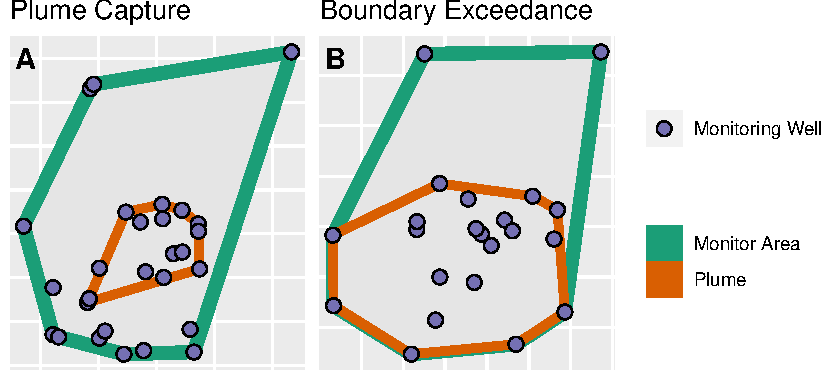
\includegraphics{CA_Benzene_Plumes_files/figure-latex/exceedsExample-1} \caption{Example of Plumes that are completely captured by monitoring wells (A) and plumes which likely travel beyond he extent of moniotring wells (B).}\label{fig:exceedsExample}
\end{figure}

\subsection{Normalizing Plume Direction}

We map the distribution of monitoring wells relative to the mean linear
direction of a benzene plume. To determine the mean linear direction of
benzene movement through the ground, we use weighted vector addition to
determine the mean angle of flow in degrees from north. We then
artificially rotate the plumes so that they are normalized to one
direction (due north) and overlay them to map out monitoring wells
relative to the leak point and direction of flow and regardless to
actual location. Coordinate math was done using the sf package
\citep{sf} and bearing directions were calculated using the stplanr
package \citep{stplanr}. Data cleaning relied on the tidyverse package
\citep{tidyverse}. To weight monitoring wells, benzene concentrations
were multiplied by the distance in meters of the monitoring well from
the LOP. Lines were then created using existing bearings for each
monitoring well from the LOP and lengths from weighted distances. Lines
were then redrawn end to end and the mean linear direction was
calculated as the bearing between the LOP and the end vertex of the
final weighted line (Figure 2).

\begin{figure}[!h]
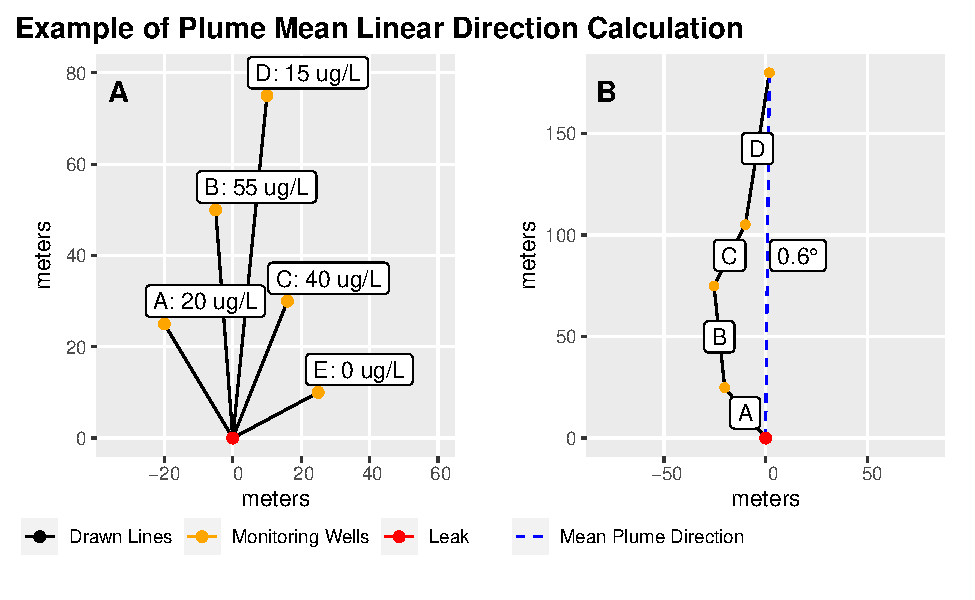
\includegraphics{CA_Benzene_Plumes_files/figure-latex/fig1-1} \caption{Illustration of mean direction calculation. Panel A shows actual locations and concentrations of benzene relative to LOP. Panel B shows weighted vector math result with mean linear direction calculation.}\label{fig:fig1}
\end{figure}

For area analyses, we included all benzene samples in Geotracker which
were taken at LUST cleanup sites and were analyzed as either ug/L or
mg/L (91.3\% of all samples). Measurements in mg/L were converted to
ug/L. In total, we included 3,495 sites which had at least 3 monitoring
wells with benzene concentrations exceeding 5 ug/L so that a
two-dimensional space could be delineated. These sites contained 63,916
spatially unique monitoring wells, with 1,545,731 benzene samples,
526,060 of which met or exceeded 5 ug/L.

\subsection{Statistical Analysis}

To determine if there is a statistically significant difference in plume
sizes depending on whether a site exhibited boundary exceedance or plume
capture we used the Wilcox test. If sites exhibiting plume capture are
significantly different then sites exhibiting boundary exceedance, it
could indicate that testing at sites that exhibit boundary exceedance
are not effectively monitoring the plumes. Finally, we show the measured
distances from the LOP for all monitoring wells used in the
two-dimensional analysis to contextualize the findings of the Wilcox
test.

\section{Results}

\subsection{Maximum Plume Distance}

Plume maximum distances were calculated for 5,624 sites which had
measurable distances (at least 2 unique monitoring wells) with
\(\ge 10 ug/L\) and 5,881 sites which had measurable distances with
\(\ge 5 ug/L\) (Figure 3). The median distance for plumes delineated at
10 ug/L was 27.7249 meters. The 90th percentile distance of plumes
delineated at 10 ug/L was 84.2 meters. The median distance for plumes
delineated at 5 ug/L was 29.42471 meters. The 90th percentile distance
of plumes delineated at 5 ug/L was 87.4 meters

Figure 3 shows the maximum distance benzene that was measured from the
point of origination. The 90th percentile for benzene distance is 595
feet for 5 ug/L which falls within the findings of \citet{connor2015}.

\begin{figure}[!h]
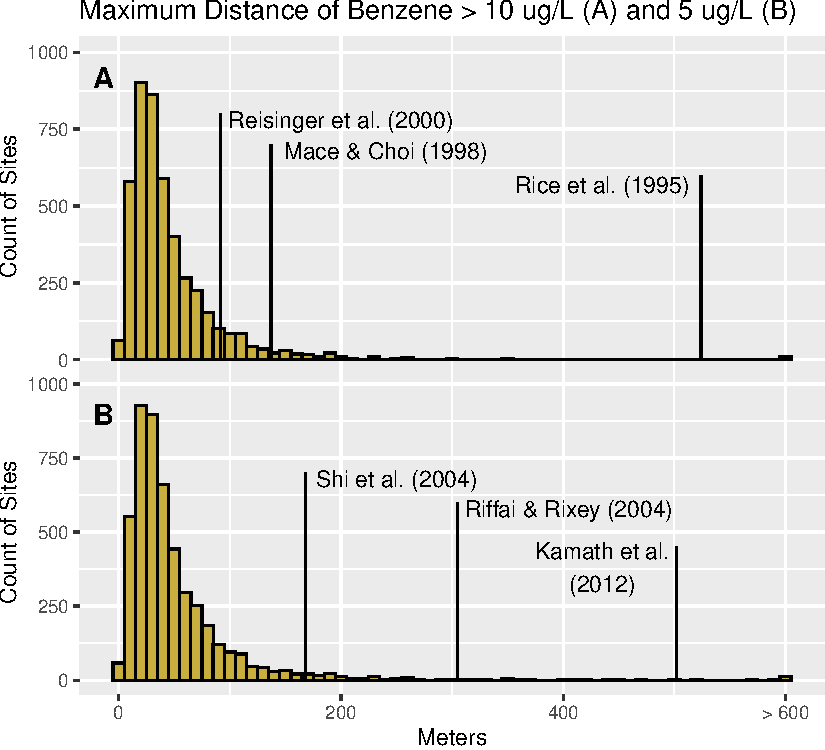
\includegraphics{CA_Benzene_Plumes_files/figure-latex/maxDistPlots-1} \caption{Histogram of maximum measured distance of benzene plumes in meters using thresholds of 10 ug/L (A) and 5 ug/L (B). Maximum distances from previous studies are overlaid. The width of bins is 10m.}\label{fig:maxDistPlots}
\end{figure}

\subsection{Directionally Normalized Plumes and Study Areas}

We found 3,495 plumes with at least 3 points with benzene concentrations
\(\ge 5 ug/L\). We calculated mean linear direction of benzene flow and
rotated each plume to due north. Each plume was overlaid by shifting the
leak origination point to the coordinates (0,0) in the California albers
projection.

\begin{figure}[!h]

{\centering 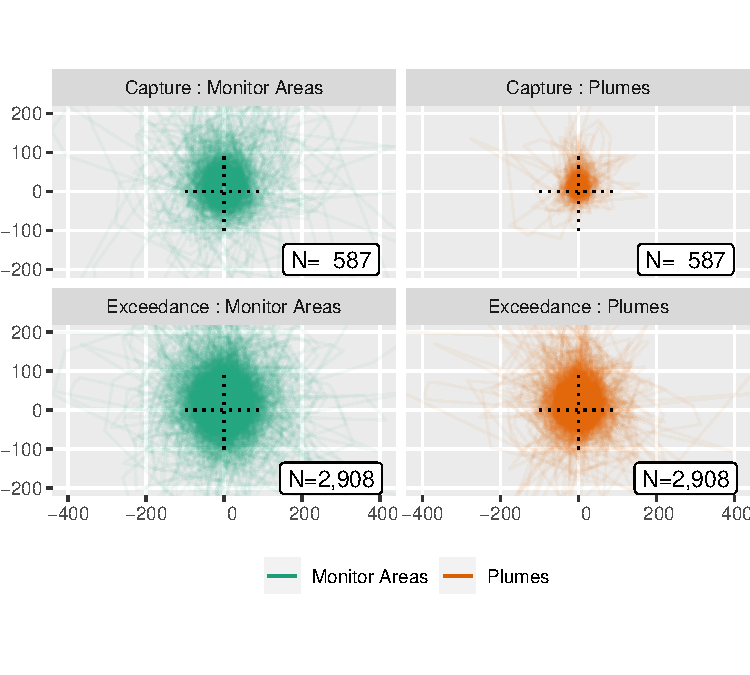
\includegraphics{CA_Benzene_Plumes_files/figure-latex/AllplumeAreas-1} 

}

\caption{Visualization of all monitoring areas and plume areas superimposed on top of eachother. Line transparency = 95 percent.}\label{fig:AllplumeAreas}
\end{figure}

\subsection{Wilcox Test}

2,908 of 3,495 cleanup sites had an exceedance of 5 ug/L at the testing
boundary (83.20458). Figure 4 illustrates that when plumes are
completely captured (spatially), they are generally smaller than if
plumes extend to the boundary of a monitoring network. The results of
the Wilcox test (Table 1) show a significant difference between the
measured plume areas at sites where boundary exceedance was observed and
at sites where entire plume capture was observed (figure 5). Plume areas
are statistically larger at sites where plumes were entirely captured,
and the majority of plumes exhibited boundary exceedance across their
monitoring well extents. The median plume area where plume capture was
observed was 416 m\textsuperscript{2}. The median plume area where
boundary exceedance was observed was 983 m\textsuperscript{2}, more than
twice as much area as plumes that were spatially captured.

\begin{figure}[!h]
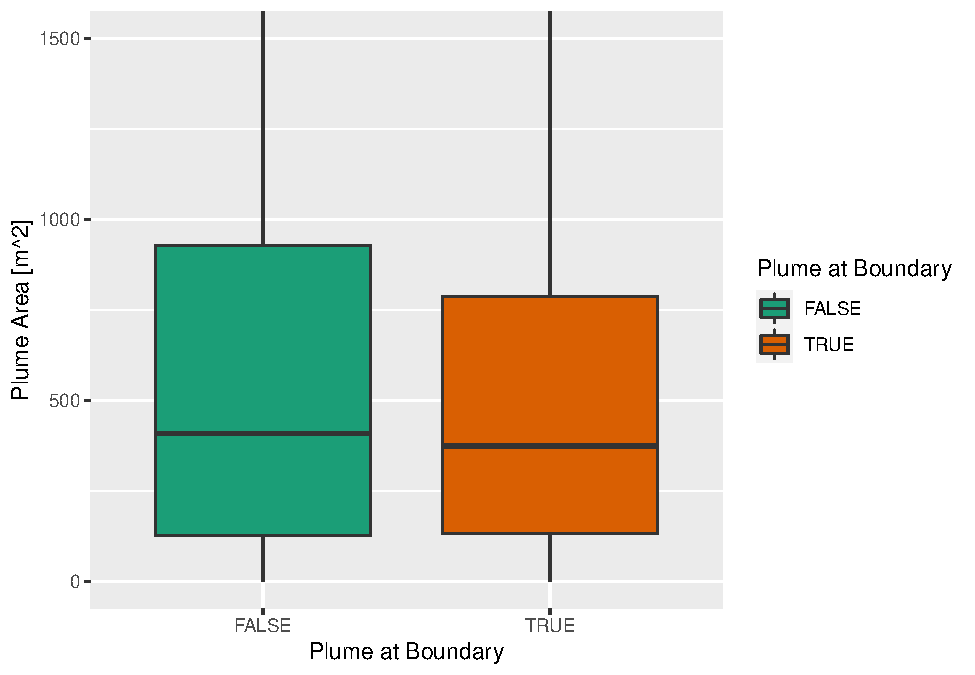
\includegraphics{CA_Benzene_Plumes_files/figure-latex/plumeAreaCompare-1} \caption{Visulization of plume areas by whether they exhibited boundary capture (green/left) or boundary exceedance (brown/right).}\label{fig:plumeAreaCompare}
\end{figure}
\begin{table}[H]

\caption{\label{tab:wilcox}Wilcox Test Results}
\centering
\begin{tabular}[t]{l|l|l|r|r|r|r|r}
\hline
Y & Group 1 & Group 2 & n1 & n2 & Statistic & p & Effect\\
\hline
Area\_m & FALSE & TRUE & 587 & 2908 & 559822 & 0 & 0.2228\\
\hline
\end{tabular}
\end{table}

\subsection{Monitoring Well Distances}

The distances of all spatially unique monitoring wells were measured
from their respective LOPs. Figure 6 shows a histogram as well as the
25th, 50th, 75th and 90th percentiles of maximuim benzene plume
distances. The median distance of all monitoring wells from the LOP was
30.03 meters. 90\% of monitoring wells were within 87.78 meters of the
LOP.

\begin{figure}[!h]
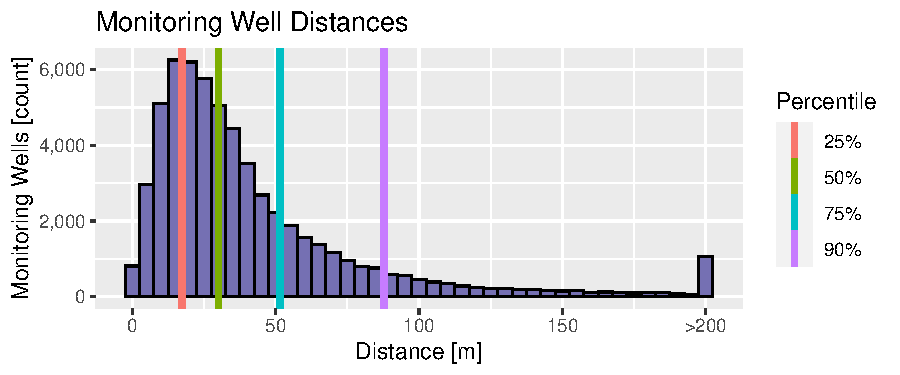
\includegraphics{CA_Benzene_Plumes_files/figure-latex/mwDistsPlot-1} \caption{Histogram of monitoring well distances used in area analysis with the 25th, 50th, 75th and 90th percentiles overlaid. Bin width = 5m}\label{fig:mwDistsPlot}
\end{figure}

\section{Conclusions \& Discussion}

While statistically, the maximum distance of 90\% of plumes falls within
the bounds of previous research, this is not necessarily the best way to
consider potential impacts of petroleum hydrocarbons in the environment.
California for example has particularly strict reporting requirements,
meaning that even very small releases are documented, and the sites
undergo soil and groundwater testing, leading to a disproportionate
weighting of plumes towards smaller releases relative to documented
releases in other states which have reporting requirements more aligned
with federal regulations. However, there are still many plumes of
concern that reach beyond the ninetieth percentile, in this case 589
sites. Further, our research finds that the vast majority of plumes
recorded are likely larger then previously thought, with maximum
distances that are longer than have been reported in the data. While
previous research has not stated whether or not plumes were entirely
captured by monitoring, it stands to reason that prior site
investigations may have suffered from the same limitations as are
present in the geotracker data. Limitations to testing often include
both physical impediments and property boundaries. For example, many gas
stations are located in urbanized areas, meaning that impervious, paved
surfaces and other structures can limit the areas where testing is
possible. Additionally, there may be several other private properties
within a very small distance, making getting permission to test
difficult. Releases can enter the ground in many ways. The release can
originate underground, directly from a tank that has suffered corrosion,
or from leaky piping connections, or it can originate on the surface
from a spill or overfill and migrate into the ground directly, or
through overland flow and via preferential pathways such as cracked
pavement.

Our findings suggest that plumes are larger than the data suggests.
Plumes are significantly larger when they are not captured by monitoring
wells, suggesting that the sites which exhibit plume capture may be
doing so simply because they are smaller in tw0-dimensional area. Larger
plumes are less likely to be completely captured because the burden for
doing so is higher. While the limitations of testing in the real world
are clear, and are not likely to be overcome in their entirety, this
research clearly shows that there is still much that is unknown about
how benzene plumes move through the environment and how much area they
can impact in unsafe levels. There is a need for better modelling and
understanding of these plumes. If we are able to more effectively model
the full extent of benzene plumes, we may be able to aid in future site
investigations without an additional burden on agencies responsible for
site testing and characterization. While on-site sampling will always be
the most reliable way to characterize a plume, additional modelling and
understanding may help future site investigations to be more efficient
by helping to prioritize monitoring well locations.

\acknowledgments

The authors of this paper have no conflicts of interest to declare. The
views expressed in this paper are those of the authors and do not
necessarily represent the views or policies of the U.S. Environmental
Protection Agency. All analysis, statistics and spatial analyses were
completed using R version 4.1.2. All California LUST data were obtained
from the California Water Board's Geotracker public portal
(https://geotracker.waterboards.ca.gov/data\_download\_by\_county). All
code used in this research is publicly available on GitHub
(https://github.com/USEPA/ORD\_Plume\_Paper).

\bibliography{references.bib}


\end{document}
